% Paper review: InfoNCE (CPC)
\documentclass{article}
\usepackage[margin=1in]{geometry}
\usepackage{amsmath,amssymb}
\usepackage{graphicx}
\usepackage[hidelinks]{hyperref}

\begin{document}

\section*{Representation Learning with Contrastive Predictive Coding (InfoNCE) (2018; v2 2019)}
\textbf{Authors:} Aaron van den Oord, Yazhe Li, Oriol Vinyals (DeepMind)\\
\textbf{PDF:} \url{https://arxiv.org/abs/1807.03748}

\begin{figure}[h]
\centering
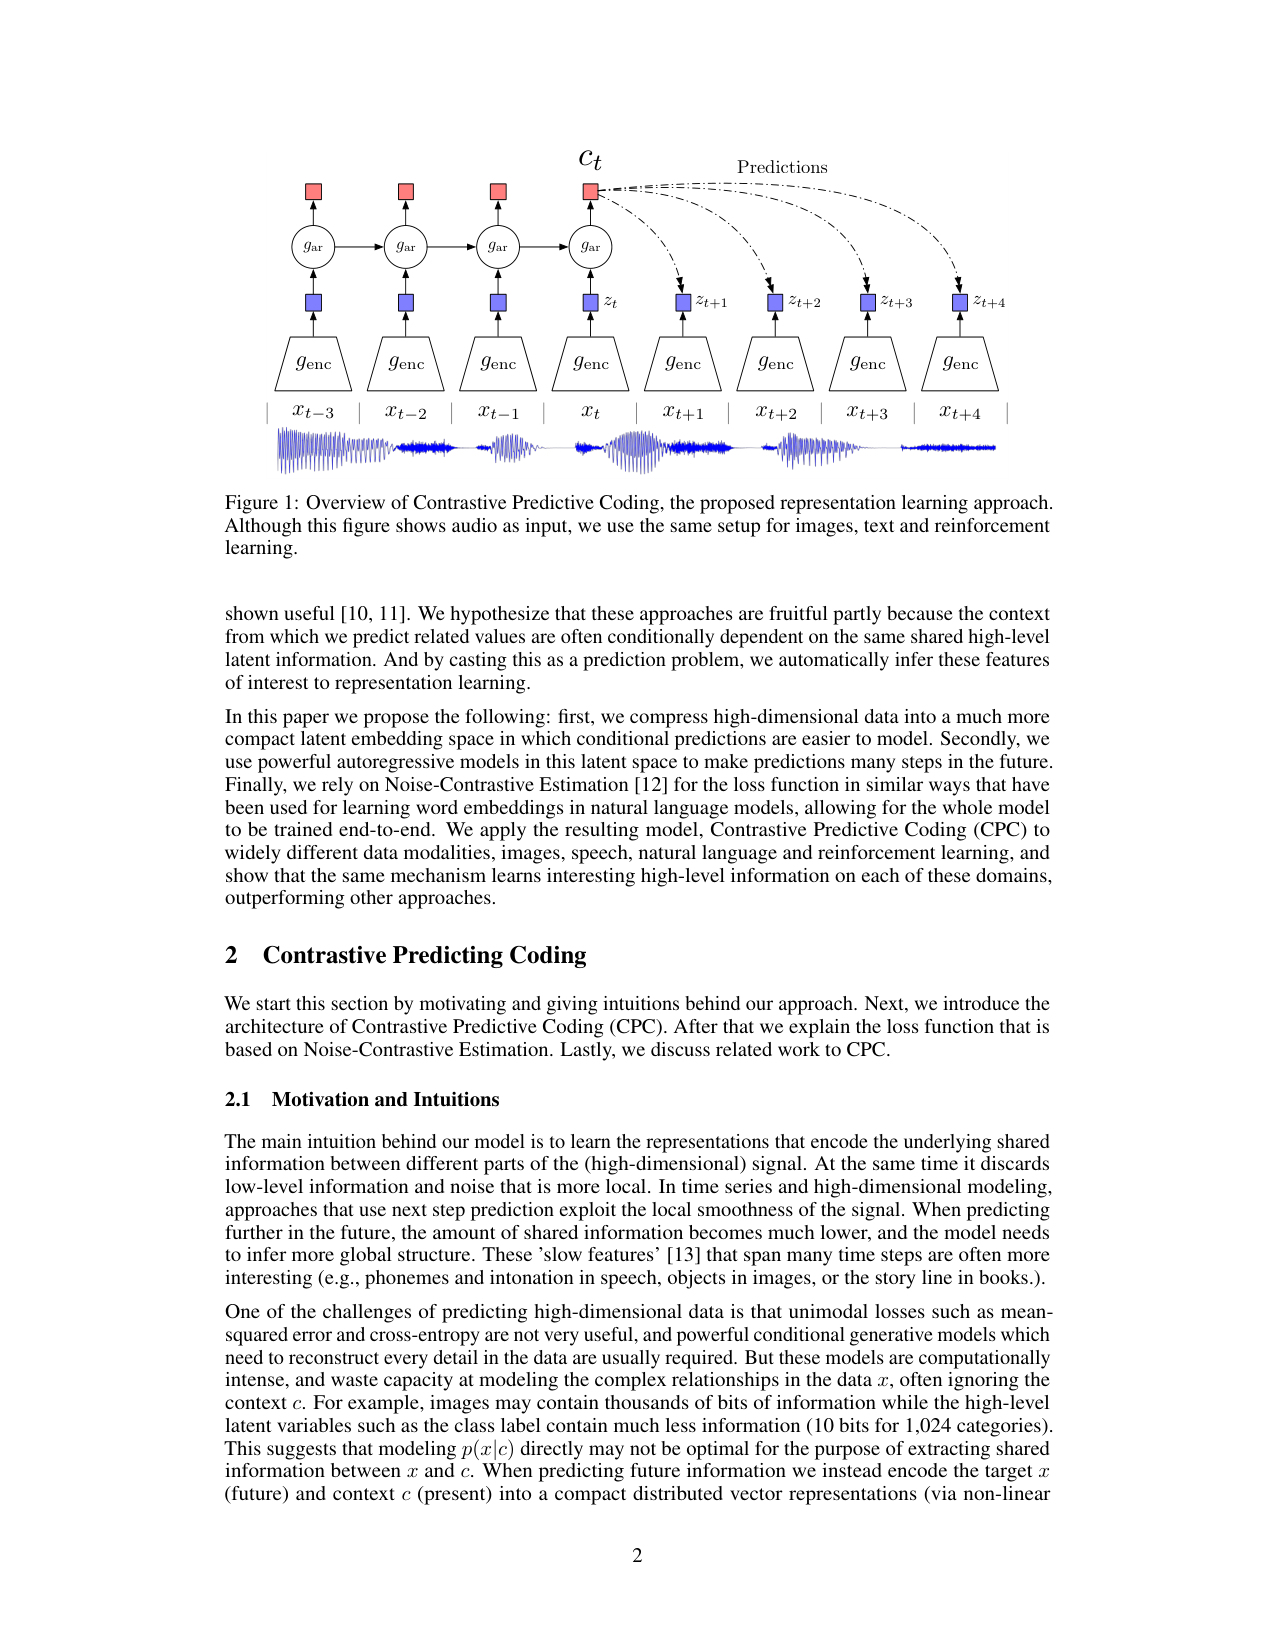
\includegraphics[width=0.95\linewidth]{fig1_cpc_overview.png}
\caption{Figure 1 (paper): overview of Contrastive Predictive Coding (CPC).}
\end{figure}

\subsection*{Challenges}
\begin{itemize}
  \item Learn representations from high-dimensional sequential data without reconstructing pixels/waveforms or relying on labels.
  \item Avoid trivial prediction objectives (too easy) or overly hard ones; create a task that forces extracting shared/high-level information over time.
  \item Scale contrastive learning stably with many negatives and across domains (speech, vision, NLP, RL).
\end{itemize}

\subsection*{Key Initiatives}
\begin{itemize}
  \item Propose CPC: encode observations into latents, summarize past with an autoregressive context, then predict future latents via a probabilistic contrastive objective.
  \item Introduce/coin \textbf{InfoNCE}: an NCE-style loss implemented as \emph{N-way classification} among one positive and many negatives.
  \item Show InfoNCE provides a mutual-information lower bound: \emph{``}$I(x_{t+k}, c_t) \ge \log(N) - L_N$\emph{''} (Sec. 2.3).
\end{itemize}

\subsection*{Methodology}
\begin{itemize}
  \item \textbf{Architecture:} encoder $g_{enc}$ maps each input $x_t \to z_t$; autoregressive model $g_{ar}$ summarizes history into context $c_t$; prediction heads score $(c_t, x_{t+k})$ pairs.
  \item \textbf{InfoNCE definition (Eq. 4):} given a set $X$ with 1 positive from $p(x_{t+k}\mid c_t)$ and $N-1$ negatives from the proposal $p(x_{t+k})$, optimize
  \[
    L_N = -\mathbb{E}\, \log \frac{f_k(x_{t+k}, c_t)}{\sum_{x_j\in X} f_k(x_j, c_t)}.
  \]
  \item The paper explicitly interprets Eq. 4 as \emph{``the categorical cross-entropy of classifying the positive sample correctly''} (Sec. 2.3), and shows the optimal scorer estimates a \textbf{density ratio} (Eq. 5).
\end{itemize}

\subsection*{InfoNCE vs other losses (key differences)}
\begin{itemize}
  \item \textbf{Vs. classic Noise-Contrastive Estimation (NCE):} CPC frames learning as NCE-style discrimination (Sec. 2.3), but InfoNCE is implemented as \textbf{multi-class (N-way) cross-entropy} over a set with 1 positive + many negatives (Eq. 4), rather than independent binary decisions. InfoNCE is also used to derive an \textbf{MI lower bound} (Sec. 2.3 / App. A.1).

  \item \textbf{Vs. triplet / max-margin ranking losses:} the paper cites prior contrastive work using \emph{``triplet losses using a max-margin approach to separate positive from negative examples''} (Sec. 2.4). Compared to margin ranking (distance + hinge), InfoNCE is \textbf{probabilistic} (softmax normalization across all negatives), giving smoother gradients and a direct interpretation as classification among candidates.

  \item \textbf{Vs. supervised cross-entropy classification:} InfoNCE uses the same mathematical form (categorical cross-entropy), but the “label” is \textbf{which element in the candidate set is the positive sample} (self-supervised), not a fixed semantic class.

  \item \textbf{Vs. maximum-likelihood generative prediction (sequence decoders):} the paper contrasts CPC’s latent predictive objective with language models that \textbf{``use maximum likelihood over sequences of observations''} (Sec. 2.4). InfoNCE avoids reconstructing raw inputs and instead learns representations by predicting \textbf{latent future information} that is shared with context.

  \item \textbf{Vs. MINE / DV-style MI estimators:} the appendix relates InfoNCE to MINE (Belghazi et al., 2018) and notes direct MINE can be \textbf{unstable when the target is easy}, whereas InfoNCE remains stable: \emph{``[MINE] became very unstable if the target was easy to predict from the context''} (App. A.1).
\end{itemize}

\subsection*{Experiments (selected)}
\begin{itemize}
  \item \textbf{Speech (LibriSpeech):} phone classification accuracy improves from 39.7 (MFCC) to 64.6 (CPC); speaker classification reaches 97.4 (Table 1).
  \item \textbf{Vision (ImageNet linear eval):} CPC reports 48.7 top-1 and 73.6 top-5 (Tables 3--4), with the text highlighting \emph{``9\% absolute''} top-1 gain over prior state of the art.
  \item \textbf{NLP (BookCorpus transfer):} comparable to Skip-thought on several tasks and strong on TREC (96.8) (Table 5).
  \item \textbf{RL (DeepMind Lab):} CPC used as an auxiliary loss improves learning curves across multiple tasks (Fig. 6).
\end{itemize}

\subsection*{References (selected; cited by the paper)}
\begin{itemize}
  \item Noise-Contrastive Estimation (Gutmann \& Hyv\"arinen, 2010; Mnih \& Teh, 2012; Mnih \& Kavukcuoglu, 2013) [12,14,15]
  \item Word2Vec negative sampling (Mikolov et al., 2013) [9]
  \item Triplet / max-margin contrastive learning (e.g., [21,22,23])
  \item PixelCNN / masked conv autoregressive modeling (van den Oord et al., 2016) [19]
  \item MINE: Mutual Information Neural Estimation (Belghazi et al., 2018) [54]
\end{itemize}

\end{document}
